\vspace*{-5mm}
\mysection{Implementation, Integration \& Test Plan}
In this section we will show the plan we have projected for implementing EasyLib. We will describe the strategy for the processes chosen for approaching the project and the structure of our team, how it is divided and the tasks that each part has to accomplish. After we will state how each team’s part has to interact with the others and the span of time of these interactions. Finally, we will supply a list of possible risks, the probability of their presence, their impact and a possible strategy to deal with them.

\mysubsection{Strategy adopted}
To give a quality assurance of the project and to be sure that the final product we have followed an Agile planning process. It consists in a first initiating part in which we have stated an overall plan application that we have implemented. We have defined the EasyLib’s requirements, discussed and stated the flow of each interaction and the specific technology to use. 
After this part, we followed the well know agility’s cycle, composed by the subsequent phases: Executing, monitoring and Controlling, Closing and Planning. Every cycle round has as input a specific process to accomplish, that is divided between the various team’s parts. After the execution of all the tasks in a precise given timeframe, the work were checked by all the parts. When the discussion on the work done has been terminated and an agreement has been reached, another planning phase containing also the corrections agreed. This cycle has been repeated until the end of the project.

\vspace*{0cm}
\begin{figure}[H]
	\centering
	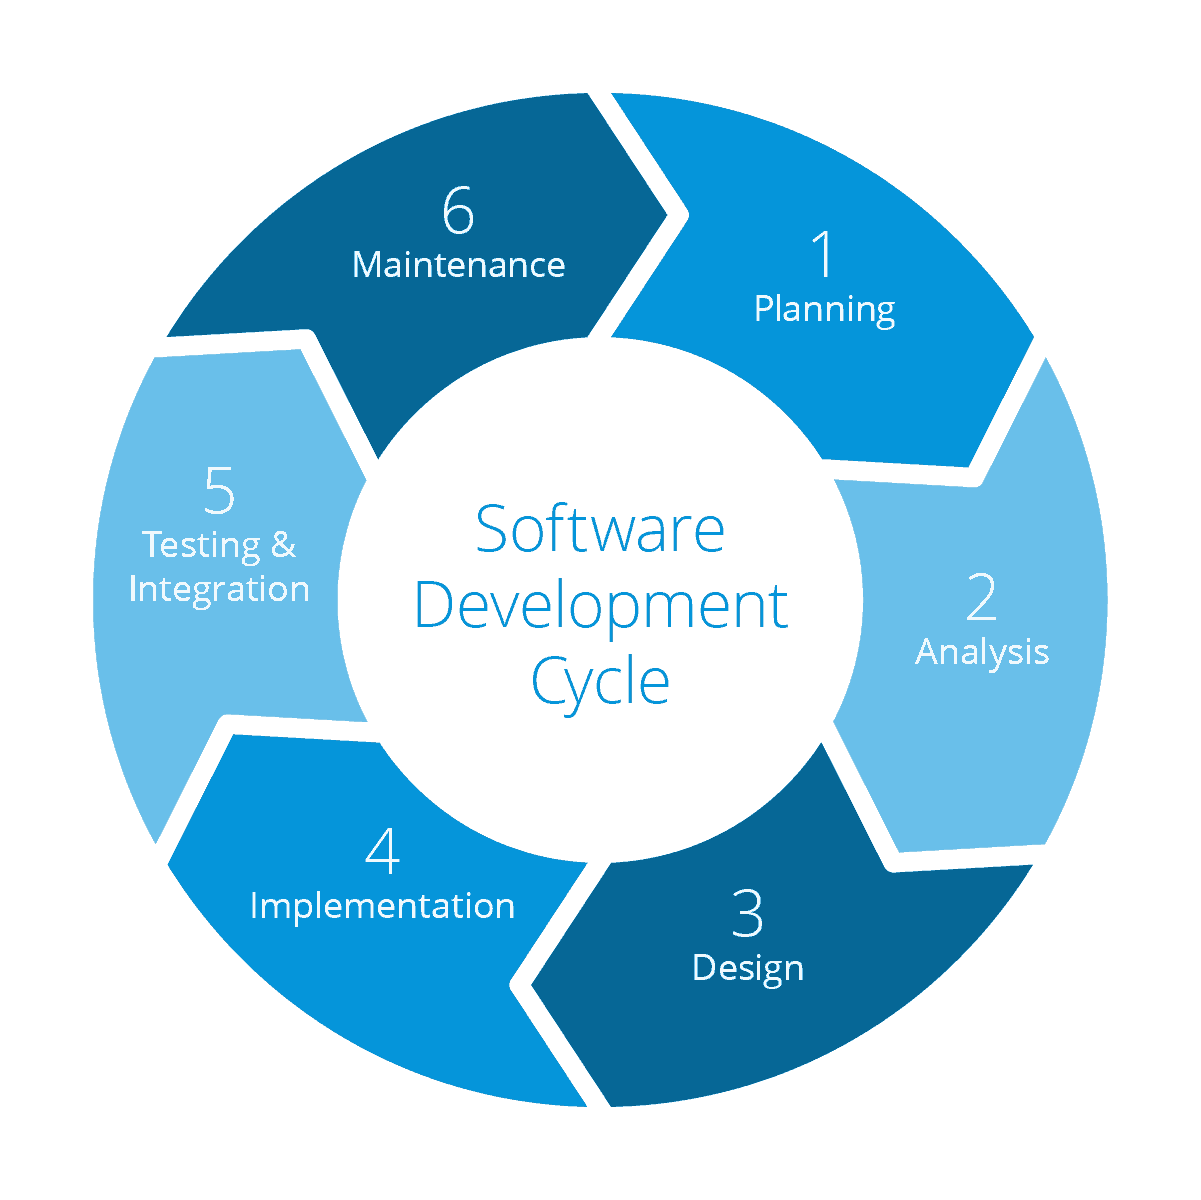
\includegraphics[scale=0.21]{Images/Diagrams/agility_cycle}
	\caption{Agility cycle}
\end{figure}

\mysubsection{Team Structure}
Our team is composed by two Computer engineers with complementary competences and that have dealt with different tasks throughout the development process. The main tasks performed are that one listed and commented right below.

\begin{itemize}
\item \emph{Client Front-End development:}this role required the full understanding of the android components related to the visualization part, the high level of image-editing software in order to produce the aimed layout and the management of the application server requests and the arrangement of the information contained in the responses to produce the whished view result. 

\item \emph{Client Back-End and Application Server development:} this role required a deep knowledge of how to build asynchronous socket multi-client network infrastructure, a good understanding in multi-table MySQL databases management, including SQL statement and trigger implementation. Nonetheless, this team component has dealt with the Android services and their communication with the application server and the main thread of the app.
\end{itemize}

\mysubsection{Implementation process}
The work has been divided in three milestones. In these spans of time the team members were required to complete the tasks that have been established in the previous planning phase. Every week a meeting to discuss about the progresses were attended and new agreement finalized to proceed at the same speed were taken. If a team’s part terminated his tasks before the milestone’s day, it usually anticipated the work programmed for the subsequent milestone but remaining ready for eventually applying changes or corrections on the software already implemented. After each milestone, some days were employed for integrating front-end and back-end part to have always a working prototype. \\
At the end of the implementation process the team has performed a Unit testing and functional testing campaign, in order to assure that all the functionalities worked correctly. Also a User acceptance test have been carried on, involving a restrict group of people which gave back feedback on their user experience that drove the developing process.

\mysubsubsection{Test cases}
As said before, in order to assure the correct behaviour of our application, we carried out tests of the main functionalities, trying to cover the wider surface of possible cases. We report below a list of the tests performed.

\begin{enumerate}
	\item 
	\begin{itemize}
		\item \emph{Goal: }Login using Email and Password
		\item \emph{Input: }The user taps on “Sign in” in Login Activity
		\item \emph{Outcome: }If the user inserts a valid email and password
		pair, after clicking on the “Sign in” button he is
		authenticated. A network connection is required to
		perform the operation
		
	\end{itemize}

\item 
\begin{itemize}
	\item \emph{Goal: }Registration using Email and Password
	\item \emph{Input: }The user inserts surname, mail, password and tap on “Register” in Register Activity
	\item \emph{Outcome: }if the user inserts a valid email, password and username, after clicking on “Register” button a new
	account is register
\end{itemize}

\item 
\begin{itemize}
	\item \emph{Goal: }Consult book information
	\item \emph{Input: }The user taps on a book object in any part of the app in which a book icon is available
	\item \emph{Outcome: }The library page is opened and all its information such as name, address, telephone number and opening time are shown to the user
	
	
\end{itemize}

\item 
\begin{itemize}
	\item \emph{Goal: }Receive notification when the user pass from the first place of the queue to have the right to take the book
	\item \emph{Input: }The user that have borrowed the book returns it to the library and the librarian confirm the transaction through the EasyLib librarian app
	\item \emph{Outcome: }The user receives a notification informing him that he can go to the library to take the book for which he was waiting for. The book become visible tapping the calendar icon on the navbar and is not more visible tapping the queue icon of the navbar. The notification is visible tapping the bell icon on the upper right part of the screen
\end{itemize}

\item 
\begin{itemize}
	\item \emph{Goal: }Search a book
	\item \emph{Input: }The user inserts title and/or author and/or category and/or library name and click on search icon
	\item \emph{Outcome: }If the book exists in one of the libraries present in the system, the books matching with the research are shown
\end{itemize}

\item 
\begin{itemize}
	\item \emph{Goal: }Reserve a copy of a book
	\item \emph{Input: }The user taps on on “reserve” button in the book page
	\item \emph{Outcome: }When the user taps on reserve, a new record in the database with the reservation’s information is created the user can consult it tapping on the calendar icon on the navbar
	
\end{itemize}

\item 
\begin{itemize}
	\item \emph{Goal: }Get in line for a book
	\item \emph{Input: }The user taps on “add queue” button in a book page
	\item \emph{Outcome: }When the user taps on “add queue”, a new record in the database with the queuing information is created and the user can consult it tapping on the queue icon on the navbar
\end{itemize}

\item 
\begin{itemize}
	\item \emph{Goal: }Register for an event
	\item \emph{Input: }The user taps on “reserve a seat” button in the event page
	\item \emph{Outcome: }When the user taps on “reserve a seat”, a new record in the database with the seat reservation information is created and the user can consult it tapping on the profile icon on the navbar
\end{itemize}

\item 
\begin{itemize}
	\item \emph{Goal: }Rate a read book
	\item \emph{Input: }The user taps on a book in the list of the read books available in the profile and set a rating between 0 and 10
	\item \emph{Outcome: }The rate is recorded in the Database, a new average rating is computed using also the new tuple and it is show to the user on the book image
\end{itemize}


\item 
\begin{itemize}
	\item \emph{Goal: }Edit profile information
	\item \emph{Input: }The user inserts new name and/or surname and/or password in the edit profile page and submit the change with a tap
	\item \emph{Outcome: }The user’s profile information is updated in the Database and the user can consult the change from the profile page
\end{itemize}

\item 
\begin{itemize}
	\item \emph{Goal: }Set a library as favourite
	\item \emph{Input: }The user taps the button “set as favourite” at the bottom of the library’s page
	\item \emph{Outcome: }The library is set as favourite for the user in the database and he can see it in the profile page or tapping on the home icon in the navbar in which he can also consult some info or the library which results to be the first that he prefers
\end{itemize}	
\end{enumerate}